\documentclass[11pt, oneside]{article} 
\usepackage{geometry}
\geometry{letterpaper} 
\usepackage{graphicx}
	
\usepackage{amssymb}
\usepackage{amsmath}
\usepackage{parskip}
\usepackage{color}
\usepackage{hyperref}

\graphicspath{{/Users/telliott/Github/calculus_book/png/}}
% \begin{center} 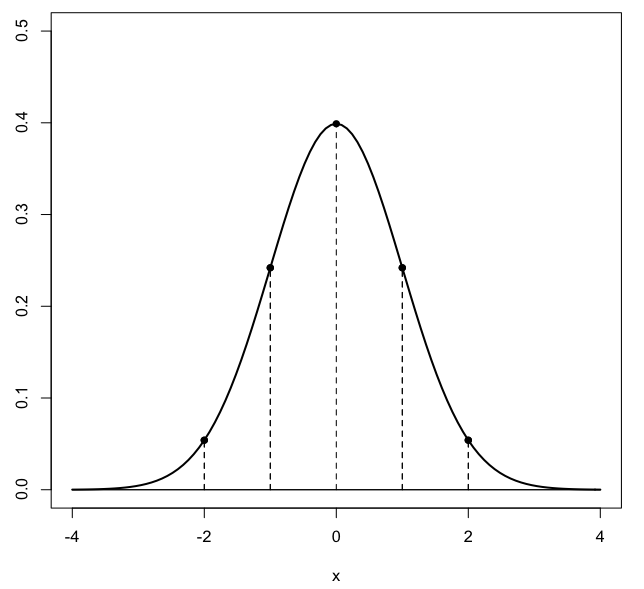
\includegraphics [scale=0.4] {gauss3.png} \end{center}

\title{Real Numbers}
\date{}

\begin{document}
\maketitle
\Large
\section*{Integers}

The \emph{natural} or counting numbers which everyone learns very early in life are $1, 2, 3$ and so on.

One can get hung up on the question of whether the natural numbers would exist without the problem of counting four sheep or all ten of our fingers.  We will not worry about that.

Mathematicians refer to the \emph{set} of natural numbers and give this set a special symbol, $\mathbb{N}$.  We write
\[ \mathbb{N} = \{ 1, 2, 3 \dots \} \]

Sometimes people say that $0 \in \mathbb{N}$ (0 is a part of the set), but most do not, and we will follow the definition given above.  To construct the set $\mathbb{N}$, start with the smallest element, $1$.  Then add successive elements by forming $a_{n+1} = a_n + 1$.

The dots mean that this sequence of numbers continue forever.  

\textbf{theorem}

$\mathbb{N}$ is an infinite set.  There is no largest number in $\mathbb{N}$, no largest $n \in \mathbb{N}$ (no largest $n$ \emph{in} $\mathbb{N}$).

Proof:  the proof is by contradiction.  Suppose $\mathbb{N}$ does have a largest number, $a$.  Well, what about $a + 1$?  By the definition we can construct it, and it is clearly also a member of the set.

A second important property of $\mathbb{N}$, as mentioned, is that there is a least number in the set.  If pairwise comparisons are carried out, a single element, the number $1$, has the property that $1 \le n$ for all numbers in $n \in \mathbb{N}$.

Since we can also find the least member of the set excluding $1$, usually written $\mathbb{N} \setminus 1$, we can order every number in $\mathbb{N}$.  

This property is called the \textbf{well-ordered} property.

The set $\mathbb{Z}$ contains all the members of $\mathbb{N}$ plus their negatives, as well as the special number $0$, often called the additive identity.

\[ \mathbb{Z} = \{ \dots -2, -1, 0, 1, 2, \dots \} \]

$\mathbb{Z}$ stands for the German word \emph{Zahlen}, Number.  The set $\mathbb{Z}$ are usually referred to as the integers.

$\mathbb{Z}$ is also an infinite set and also has the well-ordered property.  To show this simply order all numbers $p > 0$ with respect to zero using $<$, and all the numbers $n < 0$ using $>$.

\section*{Rationals}

The set $\mathbb{Q}$ (for quotient) are the rational numbers.  The name is derived from ratio.  Here is one definition, from Courant and Robbins.

\[ \mathbb{Q} = \{ \frac{p}{q} \} \text{ for } p \in \mathbb{Z}, q \in \mathbb{N} \]

Notice that we have defined $q > 0$.  If $p/q$ is to be less than zero, then it is enough that one of $p$ or $q$ be less than zero.  However, most authors don't make a big deal out of this, and going forward will just say $p,q \in \mathbb{Z}, q \ne 0$.  

$q$ must not be zero because division by zero is not defined.  We \emph{could} choose to allow division by zero, but would quickly run into logical contradictions.

\subsection*{decimal representation}

Every rational number can be represented as a decimal, using the method called long division.

Consider $1/2$
\[ 2 \overline{)1.000} \]

We say that $2$ does not \emph{go into} $1$, so we have the first part of our result as $0$, followed by a decimal point.  But $2$ does go into $10$ exactly $5$ times, giving $0.5$.  The remainder is zero and so the division process terminates.

Consider $1/8$.
\[ 8 \overline{)1.000} \]
$\circ$  $8$ goes into $10$ once, leaving $2$ as remainder

$\circ$  $8$ goes into $20$ twice, leaving $4$.  

$\circ$  $8$ goes into $40$ exactly $5$ times with no remainder.

The result is $0.125$.

The other possibility is that in going through the process a remainder comes up that has been seen previously.  If this happens then the sequence will repeat forever.

If we don't terminate with zero, then this must eventually happen, because there are only as many as $q$ possible remainders.

Thus, for example
\[ 1/7 = 0.142857142857 \dots \]

which contains $142857$, repeating.

\subsection*{decimals to fractions}

Conversely, every repeating decimal can be represented as a rational number.  For example

$1 \times r = 0.142857142857 \dots$

$1000000 \times r = 142857.142857 \dots$

$999999 \times r = 142857$

\[ r = \frac{142857}{999999} = \frac{1}{7} \]
(since $142857$ goes into $999999$ exactly $7$ times).  

You can do this trick with 

$r = 0.333 \dots$

$10 \times r = 3.33 \dots$

$9 \times r = 3$
\[ r = \frac{3}{9} = \frac{1}{3} \]

or even
$r = 0.4999 \dots$

$10*r = 4.999 \dots$

$9*r = 4.5$

\[ r = \frac{4.5}{9} = \frac{1}{2} \]

and

$r = 0.9999 \dots$

$10*r = 9.999 \dots$

$9*r = 9$

\[ r = \frac{9}{9} = 1 \]

This is one of the subtleties of numbers.  In what sense can we say that 
\[ 0.5 = 0.4999 \dots \]
\[ 1 = 0.9999 \dots \]

Most everyone is OK with the example $1/3 = 0.3333 \dots$ but some may be uneasy with the other two.

Ultimately, we justify the result as defined by evaluation of a limit.  

Consider $0.9999$.  For the number of places in the result $n \in \mathbb{N}$, then as $n \rightarrow \infty$ the number being shown approaches $1$ as its limit.  We'll come back to this after introducing the real numbers.

\subsection*{ordering}
For two rational numbers $a$ and $b$ there are only three cases:  either $a=b$, $a < b$ or $b < a$.

\[ \frac{p}{q} < \frac{s}{t} \ \iff \ pt < qs \]

$p/q$ is less than $s/t$ if and only if $pt < qs$.  Ordering of the integers guarantees ordering of the rational numbers.

Note:  we used the property that if
\[ a < b \]
then for $c > 0$
\[ ca < cb \]

\subsection*{intervals}
We denote the numbers greater than $u$ and less than $v$ as lying in the interval $(u,v)$.  With parentheses symbols, the interval described is \emph{open}, it does not include the boundary values.

To describe a \emph{closed} interval, write $[u,v]$.  This interval includes all the values in the first one, plus it also includes $u$ and $v$.

Because of the density property described below, an interval such as
\[ I = [0,1] \]
contains an \emph{infinite} quantity of rational numbers.

\subsection*{density}
Consider the set of all points
\[ x = \frac{p}{10^n} \]
for all natural numbers $n$ and integers $p$.

It is clear that simply by increasing the value of $n$, we can construct a set of equally spaced rational numbers as tightly clustered as we wish.

The rational numbers are said to be \emph{dense} on the number line.  

\subsection*{theorem}

$\bullet$  Between \emph{any} two rational numbers it is always possible to find another rational number.  

We describe this situation by writing that
\[ \forall \ u,v \in \mathbb{Q} \ \exists \ w \in \mathbb{Q} \ | \ w \in (u,v) \]
For every open interval whose bounds are rational numbers, there exists another rational number between $u$ and $v$.

Suppose we have the numbers $p/q, s/t \in \mathbb{Q}$ and that $p/q < s/t$.  The average of the two is
\[ r = \frac{1}{2} \ [ \  \frac{p}{q} + \frac{s}{t} \ ] \ = \frac{pt+sq}{2qt} \]
Thus, $r$ is rational and is equal to the average of $p/q$ and $s/t$, so it lies between them.  

More formally, as $r$ is defined above, it has the property
\[ \frac{p}{q} < r < \frac{s}{t} \]

Proof:  substitute $p/q$ for $s/t$ in the equation of the average, defining $r$ above.  The resulting number is smaller than $r$, because the substituted value is smaller than $s/t$
\[ \frac{1}{2} \ [ \  \frac{p}{q} + \frac{p}{q} \ ] \ < \frac{1}{2} \ [ \  \frac{p}{q} + \frac{s}{t} \ ] \  = r \]
but the left-hand side is equal to $p/q$.  Now do the same thing with $s/t$.
\[ r = \frac{1}{2} \ [ \  \frac{p}{q} + \frac{s}{t} \ ] \ < \frac{1}{2} \ [ \  \frac{s}{t} + \frac{s}{t} \ ]  \]

\section*{Reals}

\subsection*{unit square}

It seemed at first that a perfectly consistent system of mathematics could be built up out of only the rational numbers.  However, it was discovered that some "numbers" cannot be represented by a rational number $p/q$ with integer $p$ and $q$.

Probably the simplest example is to consider a unit square and its diagonal.  The unit square has sides of length $1$ and Pythagoras tells us that the length of the diagonal is $\sqrt{1^2 + 1^2} = \sqrt{2}$.

Clearly, this is a valid physical length (just draw the diagonal, then transfer it to the number line).

Yet as you probably know, we cannot solve the equation $(p/q)^2 = 2$ for integer $p$ and $q$ (that is, rational number $p/q$).

And generally, many numbers (defined as solutions to equations like $r^2 = 2$ or $r^2 = 3$) cannot be represented by a rational number $p/q$ with integer $p$ and $q$.  

Despite the density of the rational numbers --- recall the infinite number of rational numbers in the interval $[0,1]$, nevertheless there are values that cannot be represented as rational numbers.  This situation is described by saying that the rational number line has "holes" in it.

\subsection*{no holes}

We introduce the concept of the real numbers $\mathbb{R}$ to include all the numbers we know so far: the natural numbers, the integers, the rational numbers $p/q \in \mathbb{Q}$, \emph{plus} the irrational numbers like $\sqrt{2}$ and also $\pi$ and $e$.  In this section, when we talk about real numbers we are really exploring the properties of those real numbers which are not rational, the set $- \mathbb{Q}$. 

The discovery that one cannot find integer $p$ and $q$ such that
\[ (\frac{p}{q})^2 = 2 \]
is due to the Pythagorean school and was most unwelcome since it screwed up their cherished theory of the universe.

The standard proof is by contradiction.  We suppose that $p$ and $q$ exist with this property.  Crucially, if $p$ and $q$ have a common factor we can certainly remove it by division, so that we must start with $p/q$ already in lowest terms.

An elegant way to state this is to use the theorem which says that each number has a unique prime \emph{factorization}.  For example:
\[ 12 = 2 \times 2 \times 3 \]
\[ 256 = 2 \times 2 \times 2 \times 2 \times 2 \times 2 \times 2 \times 2 \]
\[ 4841 = 47 \times 103 \]
So for any $p$ and $q$ if they have a common factor it is certain that we can find it, and remove it by division.

Another important preliminary result is that the square of an even number is an even number.

Proof:  every (positive) even number can be expressed as $n = 2k, \ k \in \mathbb{N}$, and then

\[ n^2 = (2k)^2 = 4k^2 = 2 \cdot 2 k^2 = 2m \]
is even.  On the other hand, every (positive) odd number has an odd square because it has the form $n = 2k + 1, \ k \in \mathbb{N}$ so

\[ n^2 = (2k + 1)^2 = 2 \ [ \ 2 \cdot (k^2 + k) \ ] \  + 1 = 2m + 1 \]
and so is odd.

Returning to
\[ (\frac{p}{q})^2 = \frac{p^2}{q^2} = 2 \]
A simple rearrangement 
\[ p^2 = 2 q^2 \]
shows that $p^2$ must be even, and from the above argument, $p$ must be even.  Rewrite $p = 2p'$.  Then

\[ \frac{(2p')^2}{q^2} = 2 \]

\[ 4 p'^2 = 2 q^2 \]
\[ 2 p'^2 = q^2 \]
Hence $q^2$ is even and so is $q$, which contradicts the assumption of $p$ and $q$ as having no common factors.  

This proves that integer $p$ and $q$ with the property $p/q = \sqrt{2}$ cannot be found.

\subsection*{proof 2}

This is such an important result that we discuss another proof of it, following Stewart and Tall's \emph{The Foundations of Mathematics}.  It uses the prime factorization theorem from above.  

\textbf{Euclid's lemma} says that if a prime $p$ divides the product of two integers $a$ and $b$, then $p$ must divide at least one of $a$ and $b$.

It's a bit convoluted to prove so we will assume that part.  

From Euclid's lemma we obtain the Fundamental Theorem of arithmetic, also called the unique factorization theorem.  This says that every integer larger than 1 is either prime or is a unique product of prime factors.

Suppose $s > 1$ is the product of prime factors in two different ways:
\[ p = p_1 \cdot p_2 \dots \]
\[ q = q_1 \cdot q_2 \dots \]

By Euclid's lemma, $p_1$ must divide one of $q_1$ etc.  But these are all prime.  Therefore $p_1$ equals one of the $q_i$, say $q_1$.  Thus
\[ \frac{p}{p_1} = p_2 \dots \]
\[ \frac{p}{q_1} = q_2 \dots \]

This can be done for each of the factors $p_i$.  Therefore the factorization is unique.

Unique prime factorization can be used in turn to prove that $\sqrt{2}$ is irrational.  Since every integer $p$ is a product $p_1 p_2 \dots$, and every rational number $p/q$ is
\[ \frac{p_1 \cdot p_2 \dots}{q_1 \cdot q_2 \dots} \]
where no $p_i$ equals any $q_i$.

Every rational number squared is 
\[ \frac{p_1^2 \cdot p_2^2 \dots}{q_1^2 \cdot q_2^2 \dots} \]

But $2$ has only itself as a factor and that factor only occurs once.  There is no rational number with this property.

\section*{density}

\subsection*{number line}
A simple tool to visualize all of the real numbers is the familiar number line.  Here is the number line with numbers marked from $\mathbb{N}$, but obviously we could also draw one for $\mathbb{Z}$ or $\mathbb{Q}$.

We explore the application of the number line to $\mathbb{R}$ as we proceed.
\begin{center} 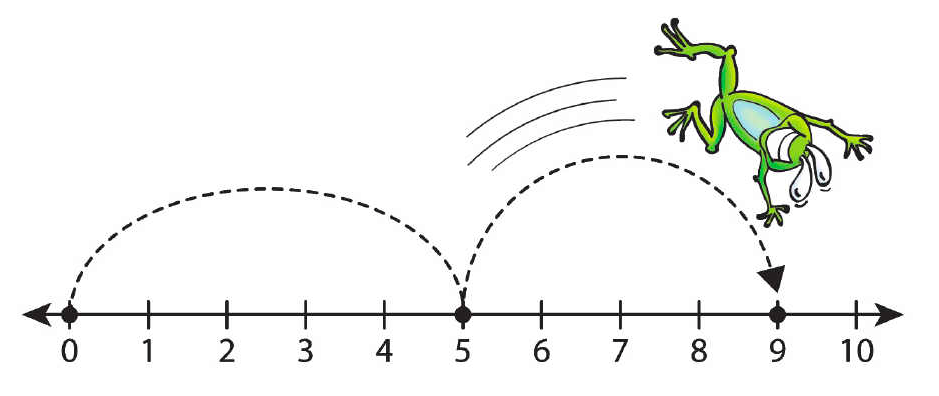
\includegraphics [scale=0.4] {number_line.png} \end{center}

We might simply assume that to every point on the number line there corresponds a rational or irrational number, and that this total collection obeys the same laws of arithmetic as the rational numbers do.

As mentioned above, the need for the real numbers is indicated by empty "holes" in the number line corresponding to the irrational numbers like $\sqrt{2}$.

A problem that arises is how to specify an irrational number non-geometrically and other than as the solution to an equation such as $r^2 = 2$.  In all cases we write particular real numbers as \emph{approximations}.  For example, the square root of $2$ lies between $1$ and $2$ because
\[ 1^2 = 1 < 2 \]
\[ 2^2 = 4 > 2 \]
Implying that $\sqrt{2} < 2$.  At the second place:
\[ 1.4^2 = 1.96 < 2 \] 
\[1.5^2 = 2.25 > 2 \]
Implying that $\sqrt{2} < 1.5$.  At the third:
\[ 1.41^2 = 1.9881 < 2 \]
\[1.42^2 = 2.0164 > 2 \]
Implying that $\sqrt{2} < 1.42$.  and at the seventh place
\[ 1.414213^2 = 1.9999984093689998.. < 2 \]
\[ 1.414214^2 = 2.0000012377960004 > 2 \]
and so on.

We can never write down the decimal value of $\sqrt{2}$ exactly, but only approximate it to greater and greater precision.  The decimal value goes on forever.  

Because any repeating decimal can be written as a fraction, we know that the sequence cannot repeat.

The real number $\sqrt{2}$ is defined to be the limit of this sequence 

$1.4, 1.41, 1.414, \dots 1.414214 \dots$ 

as the number of terms $n \rightarrow \infty$.

In a similar way, the number $e$ can be viewed as
\[ \lim_{n \rightarrow \infty} (1 + \frac{1}{n})^n \]

And the number $\pi$ can be viewed as the limit of the method of exhaustion applied to the area of a unit circle.

\end{document}